\documentclass[12pt]{article}
\usepackage[paper=a4paper,left=20mm,right=20mm,top=30mm,bottom =30mm]{geometry}
\usepackage[utf8]{inputenc}
\usepackage[T1]{fontenc}
\usepackage{stmaryrd}
\usepackage{setspace}
\usepackage{mathrsfs}
\usepackage[ngerman]{babel}
\usepackage{amssymb}
\usepackage{amsmath}
\usepackage{fancyhdr}
\usepackage[dvips,unicode,colorlinks,linkcolor=black]{hyperref} 
\usepackage{graphicx}
\usepackage{float}

\pagestyle{fancy}
\lfoot{}
\rfoot{Paul Kremser, Tobias Grussenmeyer}
\cfoot{\thepage}
\fancyhead[L]{FPI Versuch: Hanle - Effekt}
\renewcommand{\headrulewidth}{0.6pt}
\renewcommand{\footrulewidth}{0.6pt}
\setlength{\headheight}{16pt}
\setlength{\parindent}{0pt}
% Für die Wahl der Schriftart
\newcommand{\changefont}[3]{
\fontfamily{#1} \fontseries{#2} \fontshape{#3} \selectfont}

\begin{document}
% keine Hurenkinder und Schusterjungen
\clubpenalty = 10000
\widowpenalty = 10000 
\displaywidowpenalty = 10000

\onehalfspacing
% Schriftart
\changefont{ptm}{m}{n} 

\begin{titlepage}
\author{Paul Kremser, Tobias Grussenmeyer}
\title{Versuch: Hanle - Effekt}
\date{Versuchsdurchführung: 9. und 12. Oktober 2009} 
\maketitle
\thispagestyle{empty}
\end{titlepage}


\tableofcontents
\thispagestyle{empty}
\newpage
\pagenumbering{arabic}
\section{Überblick}
Mit dem Versuch soll die Lebensdauer angeregter Zustände des Queckilberatoms bestimmt werden. Grob gesagt werden hierzu Quecksilberatome in einer 
Quarzzelle durch polarisiertes Licht angeregt. Durch ein von außen angelegtes Magnetfeld wird die Richtung
in der die angeregten Atome wieder abstrahlen beeinflusst.

\section{Aufgabestellung}
Bestimmung der Lebensdauer des angeregten $6s6p \quad ^3P_1$ Zustands des $Hg$-Atoms durch Messung des Hanle-Signals in Abhängigkeit vom Dampfdruck
des Quecksilbers für verschiedene Polarisationsrichtungen des einstrahlenden Lichts. Dokumentation der Änderung der effektiven Lebensdauer durch
\textit{Coherence Narrowing}.

\section{Theoretische Grundlagen}

Wir nutzen den Hanle-Effekt zur bestimmung der Lebensdauer angeregter  Zustände im Hg-Atom. Dazu bestrahlen wir die Atome mit linear
polarisiertem Licht dessen Wellenlänge dem Übergang des zu untersuchenden Zustands entspricht. Die bestrahlten Atome werden 
dadurch angeregt und strahlen ebenfalls Licht dieser Wellenlänge und polarisation aus (Resonsnzfluoreszenz). Beobachtet man die Atome
nun aus der zur polarisation parallelen Richtung so sieht man zunächst keine Strahlung. Legt man senkrecht zur Polarisationsrichtung 
ein äusseres Magnetfeld an so sieht man bei Variation dieses Feldes auch eine Variation der Intensität. Dies wird als Hanle Effekt bezeichnet.

\subsection{Klassische Deutung}
Bei klassischer Betrachtungsweise schwingt das angeregte Atom als Dipol entlang der Polarisationsachse. Es handelt sichalso um einen gedämpften
Oszilator, das Atom schwingt bis es durch die Strahlungsdämpfung wieder zur Ruhe kommt. Betrachtet man nun diesen Dipol parallel zur 
Schwingunsachse so sieht man keine Strahlung da ein Dipol nie in dieser Richtung abstrahlt. Legt man nun senkrecht zur Schwingung ein
Magnetfeld an so beginnt das Elektron aufgrund der Lorentzkraft mit der Lamorfrequenz um die Feldrichtung zu präzedieren. Diese Frequenz 
berechnet sich zu:
\begin{align}
 \omega_L=\frac{g_j \mu_B H}{\hbar}
\end{align}
wobei $g_j$ der Landesche Faktor und $\mu_B$ das Bohrsche Magneton ist. In einer zur Feldachse senkrechten Ebene kommt
es dadurch zu einer rosettenartigen Figur der Elektronenbahn.
\\
Die Intensitätsverteilung des Dipols ist im wesentlichen eine $sin^2(\vartheta)$ Verteilung ($\vartheta$ ist der
Winkel zwischen Dipolachse und Beobachtungsrichtung). Setzt man nun $\vartheta = \omega_L t$ und beschreibt
die Dämpfung mittels denm Term $e^{-t/\tau}$, mit $\tau$ als mittlerer Lebensdauer des angeregten Zustands so 
folgt die Strahlungsintensität zu:
\begin{align}
 I = C \int \limits_{0} \limits^{\infty} e^{-\frac{t}{\tau}}sin^2(\omega_L t) dt
\end{align}

Dieses Integral ergibt augewertet eine inverse Lorentzkurve, $C$ ist eine Proportionalitätskonstante. Ist die
Polarisationsrichtung um $\pi/2$ zur Beobachtungsrichtung gedreht so ergibt sich eine normal Lorentzkurve.
In beiden Fällen gilt für die Halbwertsbreite $\omega_{\frac{1}{2}}$:
\begin{align}
 \omega_{\frac{1}{2}}= \frac{\hbar}{g_j \mu_B\tau}
\end{align}

Daraus folgt dann für die Lebensdauer, wenn $H_{\frac{1}{2}}$ die Feldstärke bei halber Höhe der vollen Intensität ist:
\begin{align}
 \label{livetime_classic} \tau = \frac{\hbar}{2 g_j \mu_B H_{\frac{1}{2}}}
\end{align}

\subsection{Quantenmechanische Deutung}
Der Hanle Effekt ist ein spezialfall des sogenanten \textit{level-crossing}. Unter level-crossing versteht man folgendes:

Liegt eine Feinstrukturaufspaltung in verschiedene Zeeman-Niveaus bereits ohne äußeres Magnetfeld vor,
so können die verschiedenen Niveaus durch Anlegen eines Feldes zur Überkreuzung gebracht werden, d. h. bei
einer bestimmten Feldstärke können zwei Niveaus energetisch zusammenfallen. In diesem Bereich findet man eine
merkliche Änderung der Intensität der Fluoreszenzstrahlung.

Der Hanle Effekt tritt bei Feldstärke null auf, d.h. die Energien der Feinstrukturauflösung fallen bei Feldstärke
null zusammen. Der Intensitätsverlauf kann quantenmechanisch hergeleitet werden, dazu kann man bei diesem Versuch die
Breit-Formel verwenden, eine Ratengleichung, welche die Absorption und Reemission von Photonen (mit der Polarisation
von $f$ bzw. $g$) in der Resonanzzelle beschreibt. Für ein System mit Grundzustand $a$ und zwei sich kreuzenden Zuständen
$b$ und $c$ lässt sich die Rate aufspalten, mit $\nu(b,c)$ als Frequenzdifferenz der angeregten Zustände.
\begin{align}
 R(f,g)=c\left[ R_0+\frac{A}{1-2\pi i \tau \nu (b,c)}+\frac{A^*}{1-2\pi i \tau \nu (b,c)}\right]
\end{align}

Man erhält für ein imaginäres A einen Intensitätsverlauf in Form einer Dispersionskurve und für ein reelles A 
eine Lorentzkurve. Von den drei Komponenten in die sich ein $^3P_1$-Term aufspaltet, nämlich $m = 0$ und $m = \pm 1$,
beobachten wir nur die Strahlung der $m = \pm1$-Komponenten. A ist in diesem Fall reell und die Energieaufspaltung im Magnetfeld beträgt:
\begin{align}
 \Delta \nu = \frac{2 g_j \mu_B H}{h}
\end{align}

Für die Halbwertsbreite der Lorentzkurve erhält man:
\begin{align}
 \Delta \nu_{\frac{1}{2}} = \frac{1}{\pi \tau} = \frac{2 g_j \mu_B 2 H_{\frac{1}{2}}}{h}
\end{align}

und somit erhält man für die mittlere Lebensdauer wieder:
\begin{align}
 \label{livetime_quantum} \tau = \frac{h}{4 g_j \mu_B \pi H_{\frac{1}{2}}} = \frac{\hbar}{2 g_j \mu_B H_{\frac{1}{2}}}
\end{align}

\subsection{Coherence Narrowing}
Hierbei handelt es sich um einen Effekt der die mittlere Lebensdauer länger erscheinen lässt. Dabei wird ein Atom in der Nähe
des angeregten durch die Strahlung des ersteren selbst angeregt. Dieses Schwingt unter Beibehaltung der Präzession, Phase und
Raumorientierung der Dipolschwingung des ersten Atoms. Dieser Prozess kann mehrfach auftreten, seine Wahrscheinlichkeit hängt
vom Dampfdruck der beobachteten Substanz ab. Der Dampdruck steigt mit der Temperatur, wesshalb wir Messungen bei verschiedenen
Temperatur durchführen um dann auf den Wert $T=0K$ zu extrapolieren.
\newpage

\section{Versuchsaufbau}
\begin{figure}[H]  
\centering
%\includegraphics[width=0.7\linewidth]{pictures/Aufbau.ps}
\caption{Versuchsaufbau des Hanle-Effekts}
\end{figure}

Als Lichtquelle dient eine HF-induzierte Gasentladung in einer Quecksilberdampflampe. Das Lich gelangt über zwei Linsen, 
einem Interferenzfilter und einem Polarisator in die mit Quecksilberdampf gefüllte Resonanzzelle aus Quarz. Die erste Linse 
macht das Licht parallel, der Interferenzfilter filtert die zur Anregung des $^3P_1$-Zustands benötigte Spektrallinie, der 
Polarisator polarisiert das Licht in die gewünschte Richtung und die zweite Linse fokussiert das Licht in die Zelle. Die Zelle
wird über ein Kühlsystem aus Peltierelement und Wasserkühlung gekühlt um die Messung bei verschiedenen Temperaturen (also
verschiedenen Dampfdrücken) zu ermöglichen. Um die Zelle herum sind drei Helmholtzspulenpaare angebracht. Zwei davon sind
zur Kompenstion der von externen (u.a. Erdamgnetfeld) Stöhrfeldern, das dritte ist zum erzeugen des für den Hanle Effekt 
nötigen Magnetfeldes, dieses wird wärend des Versuchs variiert. Senkrecht zur Einfallsrichtung des Lichts wird die erzeugte
Resonanzstrahlung Über einen Lichtleiter zum Photomultiplier geführt. Von dort wird das Signal an ein Elektrometer
weitergegeben, das über ein Osziloskop an einen Computer angeschlossen ist, mit dem das Signal dann aufgezeichnet wird.
\newpage

\section{Durchführung}
Zunächst stellten wir die kompensierenden Magnetfelder ein und justierten den Polarisator auf $90^\circ$. Wir erhielten
ein sauberes symetrisches Hanle Signal. Dann kühlten wir Die Resonanzzelle auf die minimal ereichbare Temperatur ab. Die
Temperaturmessung erwies sich als äußerst schwierig: Die in dier Anleitung beschriebene Temperaturanzeige am Peltiernetzgerät
war nicht vorhanden. Das vohandene Digitalthermometer wurde jedoch durch die Hochfrequenz der Lampe gestört. Zudem konnte das
Digitalthermometer die Temperatur nur auf $1^\circ$C anzeigen. Um eine bessere Auflösung der Temperatur zu erhalten stellten wir
die Anzeige auf Fahrenheit um ($1^\circ$C = $5/9^\circ$F). Da die Störung durch die Lampe während der Messung nicht zu vermeiden
war überprüften wir die Temperatur jeweils vor und nach einer Messreihe bei ausgeschalteter Lampe. Zunächst erreichten wir eine
minimale Temperatur von $-11^\circ$C und nahmen wärend des Aufwärmens Messungen bis $10^\circ$C auf. Danach justierten wir den
Polarisator auf $\pm 45^\circ$ und nahmen je eine Dispersionskurve auf. Zuletzt kühlten wir wieder (über 3 Stunden, laut Anleitung wird
nach einer Stunde die minmale Temperatur erreicht) um die $0^\circ$-Polarisationrichtung zu vermessen. Leider erreichten
wir hier nur noch eine Temperatur von $-8^\circ C$. 

\section{Auswertung}
Die genutzte Formel zum fitten der Lorentzkurve lautet:
\begin{align}
 y(x) &= y_0+\frac{2A}{\pi}\frac{\omega}{4(x-x_c)^2+\omega^2}+b_x \\
\notag \textnormal{ mit }~~~~ y_0~&\widehat{=} \textnormal{ Y-Achsenoffset } \\
\notag A~ &\widehat{=} \textnormal{ Fläche } \\
\notag x_0~ &\widehat{=} \textnormal{ X-Koordinate des Peaks } \\
\notag \omega~ &\widehat{=} \textnormal{ Halbwertsbreite der Kurve } \\
\notag b~ &\widehat{=} \textnormal{ Steigung des linearen Terms zur berücksichtigung der Temperatur}
\end{align}

Bei den zum Fitten verwendeten Messpunkten beschränkten wir uns auf einen Bereich von $0,7A$ um den Peak der Kurve, um
Unregelmässigkeiten am Rand der Messung auszufiltern. Der Parameter $\omega$ dieser Kurve liefert uns direkt die
Halbwertsbreite in Ampère. Aus dieser können wir die Magnetfeldstärke $H_{\frac{1}{2}}$ in Tesla bei halber Intensität bestimmen:
\begin{align}
 2H_{\frac{1}{2}}= 3,363\cdot 10^{-4} \omega
\end{align}

Also folgt mit Gleichung \ref{livetime_classic} oder \ref{livetime_quantum} die Lebensdauer in Sekunden:
\begin{align}
 \tau = \frac{\hbar}{2g_j \mu_B H_{\frac{1}{2}}} = \frac{\hbar}{g_j \mu_B\cdot 3,363\cdot 10^{-4} \omega}
\end{align}

mit dem Fehler:
\begin{align}
 s_{\tau}=\tau \frac{s_{\omega}}{\omega}
\end{align}

Für die Fits haben wir jeweils nur eine Beispielgrafik angeführt. Die ergebnisse der 74 einzelnen Fits sind im Anhang in zwei Tabellen zusammengefasst.

\begin{figure}[H]  
\centering
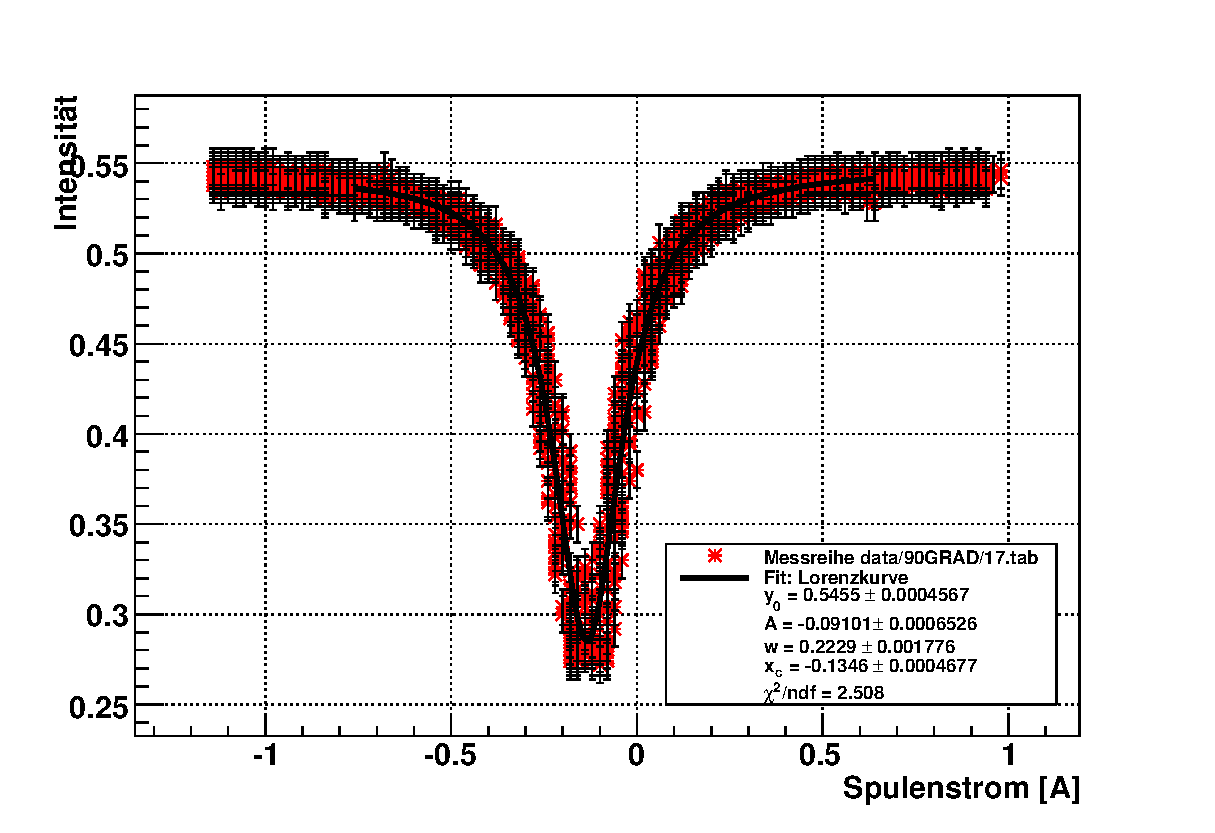
\includegraphics[width=0.9\linewidth]{pictures/9017eps.eps}
\caption{Beispiel eines Fits für die $90^\circ$ Messung}
\end{figure}

\begin{figure}[H]  
\centering
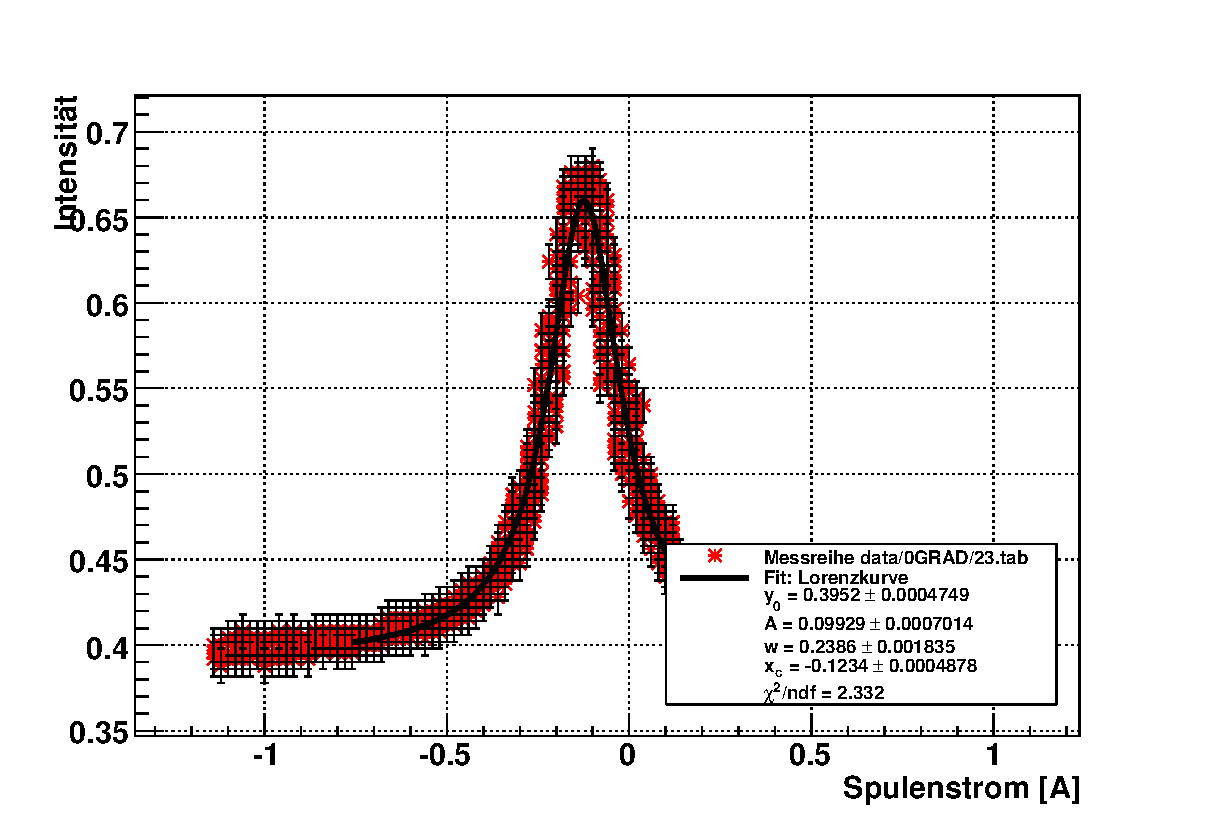
\includegraphics[width=0.9\linewidth]{pictures/023eps.eps}
\caption{Beispiel eines Fits für die $0^\circ$ Messung}
\end{figure}

\begin{figure}[H]  
\centering
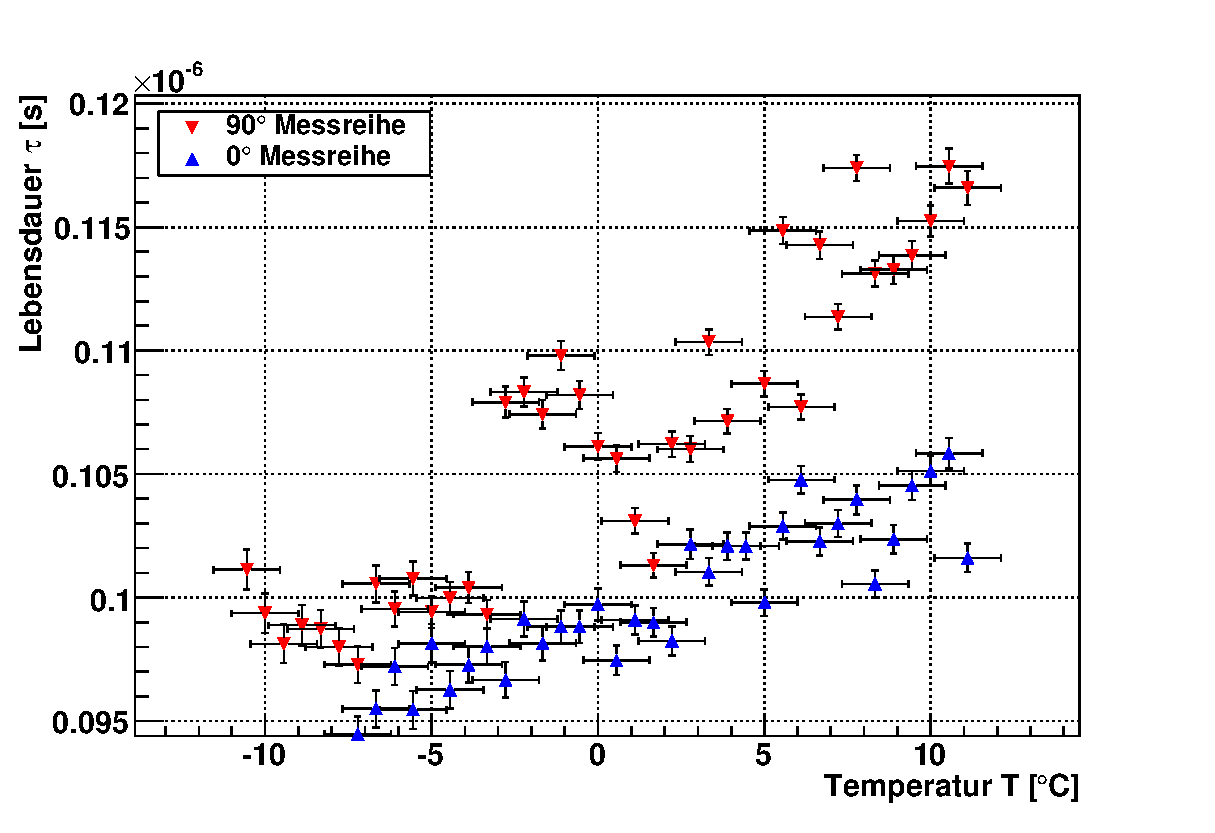
\includegraphics[width=0.9\linewidth]{pictures/lebensdauer_temp.eps}
\caption{Lebensdauer nach Temperatur}
\label{leben_temp}
\end{figure}

Die in Fahrenheit gemessenen Temperaturen haben wir zu beginn in Celsius umgerechnet:
\begin{align}
 T_{^\circ C} = (T_{^\circ F} - 36) \cdot 5 / 9
\end{align}

Den Fehler auf die in Fahrenheit gemessene Temperatur haben wir mit $1^\circ F$ angenommen. Somit ergibt sich für den Fehler auf die Temperatur in
$^\circ C$: $s_{T_{^\circ C}} = 5 / 9 ^\circ C$.

Nun trugen wir die errechneten Lebensdauern gegen die Temperatur auf (siehe Abb.\ref{leben_temp}). In der Grafik kann man schön das 
\textit{coherence narrowing} beobachten.

Um aus der Temperatur (in Kelvin) den Dampfdruck $p$ (in $Torr$) zu bestimmen verwendeten wir die in der Anleitung angegebene Formel:
\begin{align}
 log_{10}(p/Torr) = A + B ~ log_{10}(T/K) + \frac{C}{T}
\end{align}

Verwendete Konstanten: \\
\begin{tabular}{|c|c|c|c|}
 \hline
 Temperaturbereich&$A$&$B$&$C$\\
 \hline
 $T = -30^\circ C \cdots +3^\circ C$&$8,86$&$0$&$-3340K$ \\
 $T = +3^\circ C \cdots +25^\circ C$&$10,5724$&$-0,847$&$-3342,26K$ \\
 \hline
\end{tabular}

Für den Fehler ergibt sich : fehlt noch

Schliesslich konnten wir die Lebensdauern gegen den Dampfdruck auftragen und mit linearer Regression auf die natürliche Lebensdauer extrapolieren.

\begin{figure}[H]  
\centering
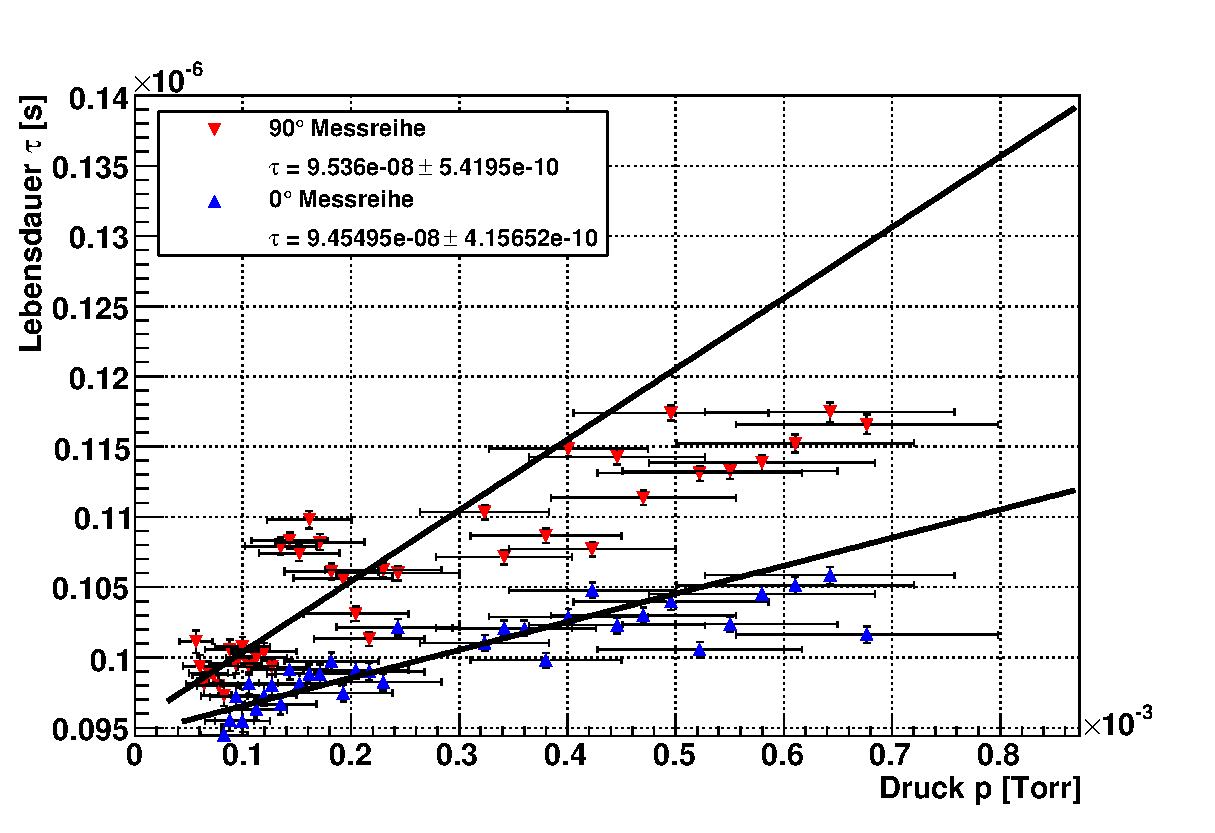
\includegraphics[width=0.9\linewidth]{pictures/lebensdauer_druck.eps}
\caption{Lebensdauer nach Druck}
\end{figure}

Für die Messung bei $90^\circ$ erhielten wir so:
\begin{align}
 \tau_{90^\circ} = (0,9772 \pm 0,0024) \cdot 10^{-7}
\end{align}

und für $0^\circ$:
\begin{align}
 \tau_{0^\circ} = (0,9552 \pm 0,0025) \cdot 10^{-7}
\end{align}


\begin{figure}[H]  
\centering
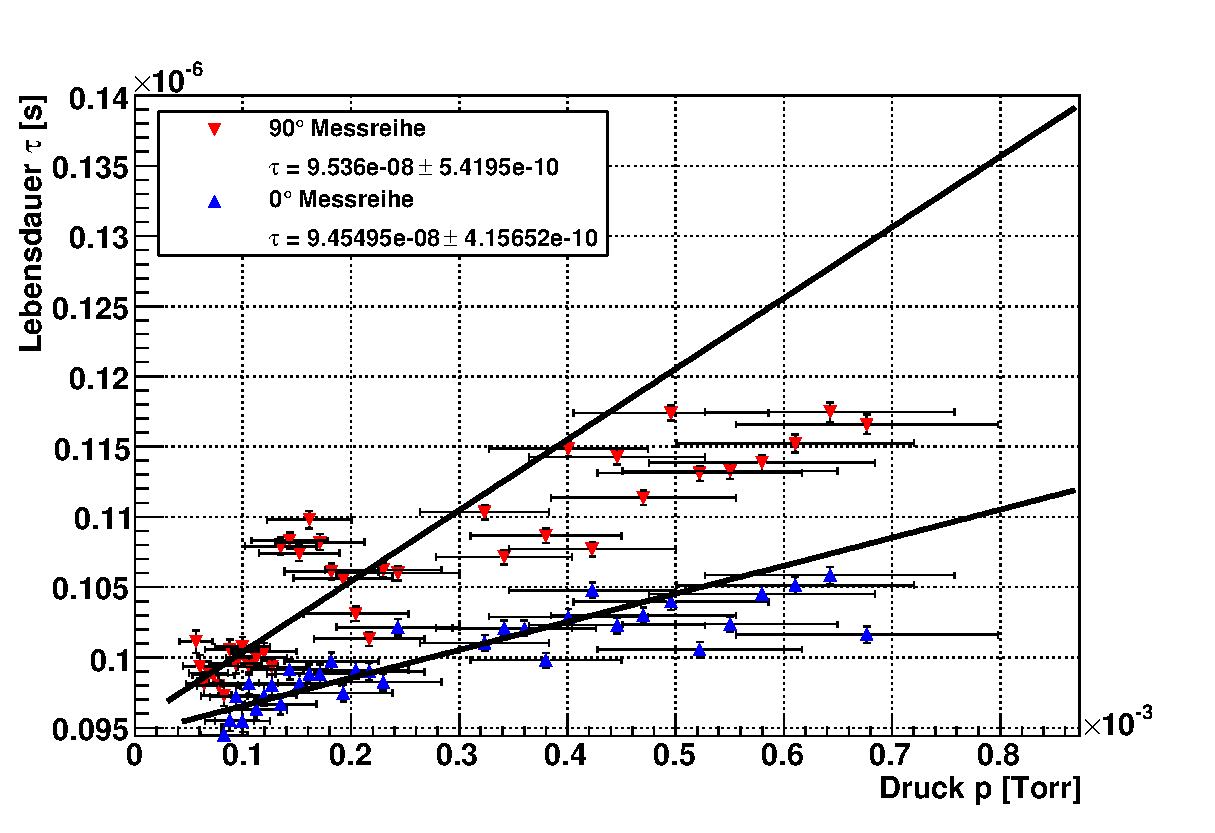
\includegraphics[width=0.9\linewidth]{pictures/lebensdauer_druck.eps}
\caption{Dispersionskurve bei $45^\circ$}
\end{figure}

Die Grafik von einer der Messungen bei $45^\circ$ zeigt den Typischen Verlauf einer Dispersionskurve.






\section{Zusammenfassung}

\section{Anhang}
\singlespacing
\centering
\textbf{$90^\circ$} \\

\begin{tabular}{|c|c|c|c|c|c|}
\hline
Messung&$\chi^2/ndf$&$w\;/A$&$s_w\;/A$&$\tau\;/10^{-7}s$&$s_{\tau}\;/10^{-7}s$\\
\hlinedata/90GRAD/17.tab&2.508230&0.222897&0.001776&1.011315&0.008058 \\
data/90GRAD/18.tab&2.451964&0.226857&0.001850&0.993661&0.008103 \\
data/90GRAD/19.tab&2.746109&0.229712&0.001864&0.981311&0.007963 \\
data/90GRAD/20.tab&3.041531&0.227988&0.001893&0.988732&0.008210 \\
data/90GRAD/21.tab&3.219703&0.228329&0.001794&0.987255&0.007757 \\
data/90GRAD/22.tab&3.079926&0.230042&0.001775&0.979904&0.007561 \\
data/90GRAD/23.tab&3.335248&0.231721&0.001744&0.972804&0.007322 \\
data/90GRAD/24.tab&2.954065&0.224162&0.001650&1.005608&0.007402 \\
data/90GRAD/25.tab&2.906293&0.226452&0.001634&0.995438&0.007183 \\
data/90GRAD/26.tab&3.131300&0.223700&0.001527&1.007685&0.006879 \\
data/90GRAD/27.tab&3.333265&0.226741&0.001457&0.994170&0.006388 \\
data/90GRAD/28.tab&4.294901&0.225475&0.001455&0.999752&0.006451 \\
data/90GRAD/29.tab&3.941493&0.224511&0.001397&1.004044&0.006248 \\
data/90GRAD/30.tab&4.101223&0.226959&0.001297&0.993215&0.005676 \\
data/90GRAD/31.tab&4.656507&0.208915&0.001201&1.078999&0.006203 \\
data/90GRAD/32.tab&4.696823&0.208117&0.001135&1.083136&0.005907 \\
data/90GRAD/33.tab&4.678136&0.209857&0.001120&1.074155&0.005733 \\
data/90GRAD/34.tab&4.453375&0.205310&0.001119&1.097945&0.005984 \\
data/90GRAD/35.tab&5.227775&0.208349&0.001094&1.081930&0.005681 \\
data/90GRAD/36.tab&7.225497&0.212452&0.001094&1.061035&0.005464 \\
data/90GRAD/37.tab&8.230502&0.213422&0.001037&1.056213&0.005132 \\
data/90GRAD/38.tab&8.708958&0.218647&0.001101&1.030972&0.005191 \\
data/90GRAD/39.tab&9.624258&0.222524&0.001094&1.013010&0.004980 \\
data/90GRAD/40.tab&7.347724&0.212245&0.001031&1.062070&0.005159 \\
data/90GRAD/41.tab&9.069906&0.212668&0.001045&1.059957&0.005208 \\
data/90GRAD/42.tab&8.579667&0.204312&0.000967&1.103308&0.005222 \\
data/90GRAD/43.tab&8.268835&0.210424&0.000981&1.071261&0.004994 \\
data/90GRAD/45.tab&9.916675&0.207493&0.000985&1.086393&0.005157 \\
data/90GRAD/46.tab&7.076396&0.196285&0.000933&1.148427&0.005459 \\
data/90GRAD/47.tab&9.367823&0.209302&0.000990&1.077004&0.005094 \\
data/90GRAD/48.tab&9.043662&0.197305&0.000959&1.142490&0.005553 \\
data/90GRAD/49.tab&9.368138&0.202441&0.000946&1.113505&0.005203 \\
data/90GRAD/50.tab&7.610235&0.192043&0.000863&1.173795&0.005275 \\
data/90GRAD/51.tab&9.065930&0.199313&0.000942&1.130980&0.005345 \\
data/90GRAD/52.tab&7.953311&0.199018&0.001031&1.132656&0.005868 \\
data/90GRAD/53.tab&8.655581&0.198013&0.000938&1.138405&0.005393 \\
data/90GRAD/54.tab&7.604723&0.195621&0.001065&1.152325&0.006273 \\
data/90GRAD/55.tab&8.307936&0.191939&0.001143&1.174431&0.006994 \\
data/90GRAD/56.tab&7.401482&0.193380&0.001124&1.165679&0.006775 \\
\hline
\end{tabular}
\newpage
\textbf{$0^\circ$} \\

\begin{tabular}{|c|c|c|c|c|c|}
\hline
Messung&$\chi^2/ndf$&$w\;/A$&$s_w\;/A$&$\tau\;/10^{-7}s$&$s_{\tau}\;/10^{-7}s$\\
\hlinedata/0GRAD/23.tab&2.332279&0.238602&0.001835&0.944749&0.007266 \\
data/0GRAD/24.tab&2.345471&0.236021&0.001847&0.955080&0.007474 \\
data/0GRAD/25.tab&1.880115&0.231891&0.001767&0.972090&0.007407 \\
data/0GRAD/26.tab&2.360273&0.236129&0.001908&0.954644&0.007714 \\
data/0GRAD/27.tab&1.974942&0.229680&0.001827&0.981448&0.007807 \\
data/0GRAD/28.tab&1.834960&0.234156&0.001758&0.962687&0.007228 \\
data/0GRAD/29.tab&2.019624&0.231699&0.001733&0.972896&0.007277 \\
data/0GRAD/30.tab&2.177508&0.229960&0.001739&0.980253&0.007413 \\
data/0GRAD/31.tab&2.040100&0.233185&0.001715&0.966696&0.007110 \\
data/0GRAD/32.tab&2.540441&0.227379&0.001630&0.991380&0.007107 \\
data/0GRAD/33.tab&2.424776&0.229678&0.001618&0.981457&0.006914 \\
data/0GRAD/34.tab&2.442114&0.228117&0.001525&0.988173&0.006606 \\
data/0GRAD/35.tab&2.607706&0.228124&0.001514&0.988143&0.006558 \\
data/0GRAD/36.tab&2.646193&0.226062&0.001442&0.997156&0.006361 \\
data/0GRAD/37.tab&3.166693&0.231305&0.001424&0.974553&0.006000 \\
data/0GRAD/38.tab&3.283183&0.227469&0.001358&0.990988&0.005916 \\
data/0GRAD/39.tab&3.175862&0.227715&0.001343&0.989917&0.005838 \\
data/0GRAD/40.tab&3.980025&0.229446&0.001354&0.982449&0.005798 \\
data/0GRAD/41.tab&4.083944&0.220664&0.001282&1.021549&0.005935 \\
data/0GRAD/42.tab&3.856461&0.223098&0.001244&1.010404&0.005634 \\
data/0GRAD/43.tab&4.289890&0.220838&0.001215&1.020744&0.005616 \\
data/0GRAD/44.tab&4.074276&0.220835&0.001183&1.020758&0.005468 \\
data/0GRAD/45.tab&5.064290&0.225875&0.001228&0.997981&0.005426 \\
data/0GRAD/46.tab&5.065020&0.219089&0.001211&1.028892&0.005687 \\
data/0GRAD/47.tab&4.706524&0.215159&0.001160&1.047686&0.005648 \\
data/0GRAD/48.tab&4.831626&0.220405&0.001211&1.022749&0.005619 \\
data/0GRAD/49.tab&4.987142&0.218874&0.001176&1.029903&0.005534 \\
data/0GRAD/50.tab&5.198148&0.216858&0.001200&1.039478&0.005752 \\
data/0GRAD/51.tab&7.113286&0.224200&0.001218&1.005437&0.005462 \\
data/0GRAD/52.tab&5.123523&0.220219&0.001229&1.023613&0.005713 \\
data/0GRAD/53.tab&5.143762&0.215657&0.001211&1.045266&0.005870 \\
data/0GRAD/54.tab&3.838946&0.214433&0.001234&1.051233&0.006050 \\
data/0GRAD/55.tab&3.949027&0.212983&0.001236&1.058390&0.006142 \\
data/0GRAD/56.tab&4.878466&0.221853&0.001267&1.016074&0.005803 \\
\hline
\end{tabular}
\newpage
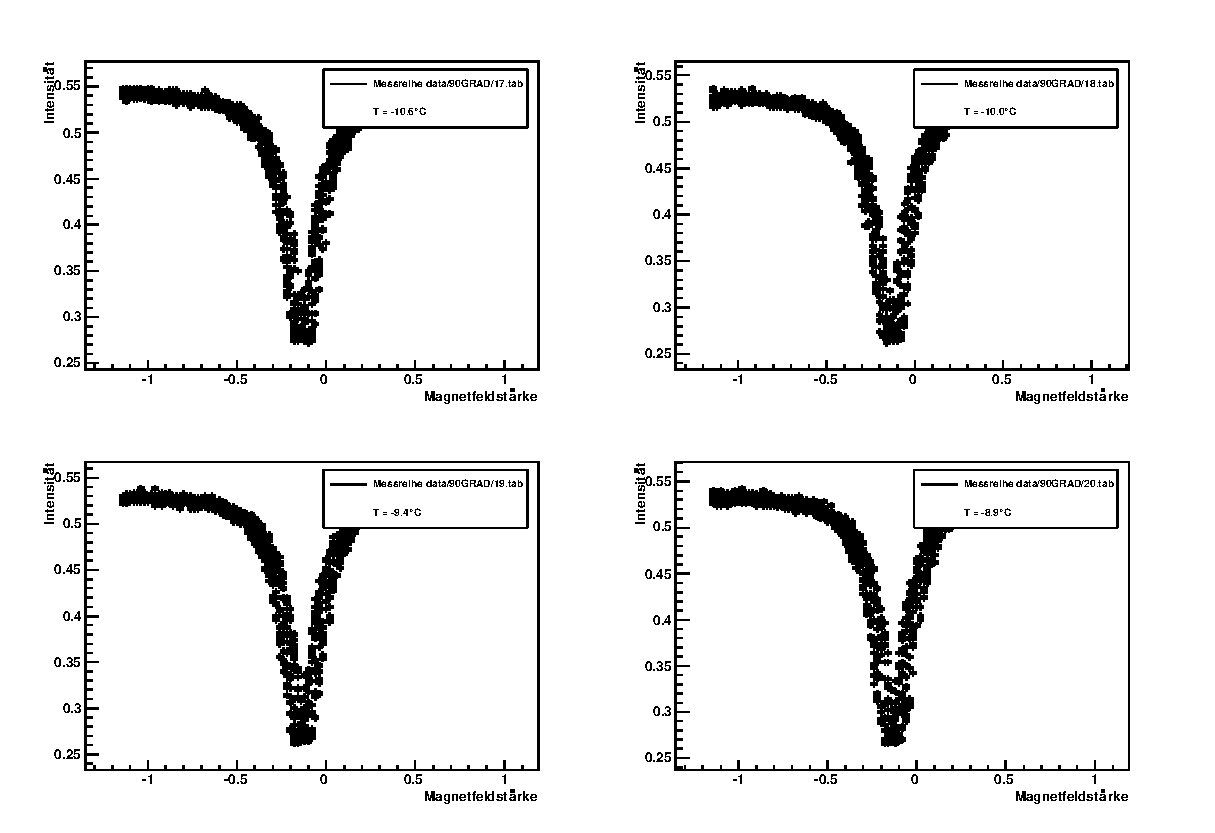
\includegraphics[width=1\linewidth]{pictures/1.eps} \\
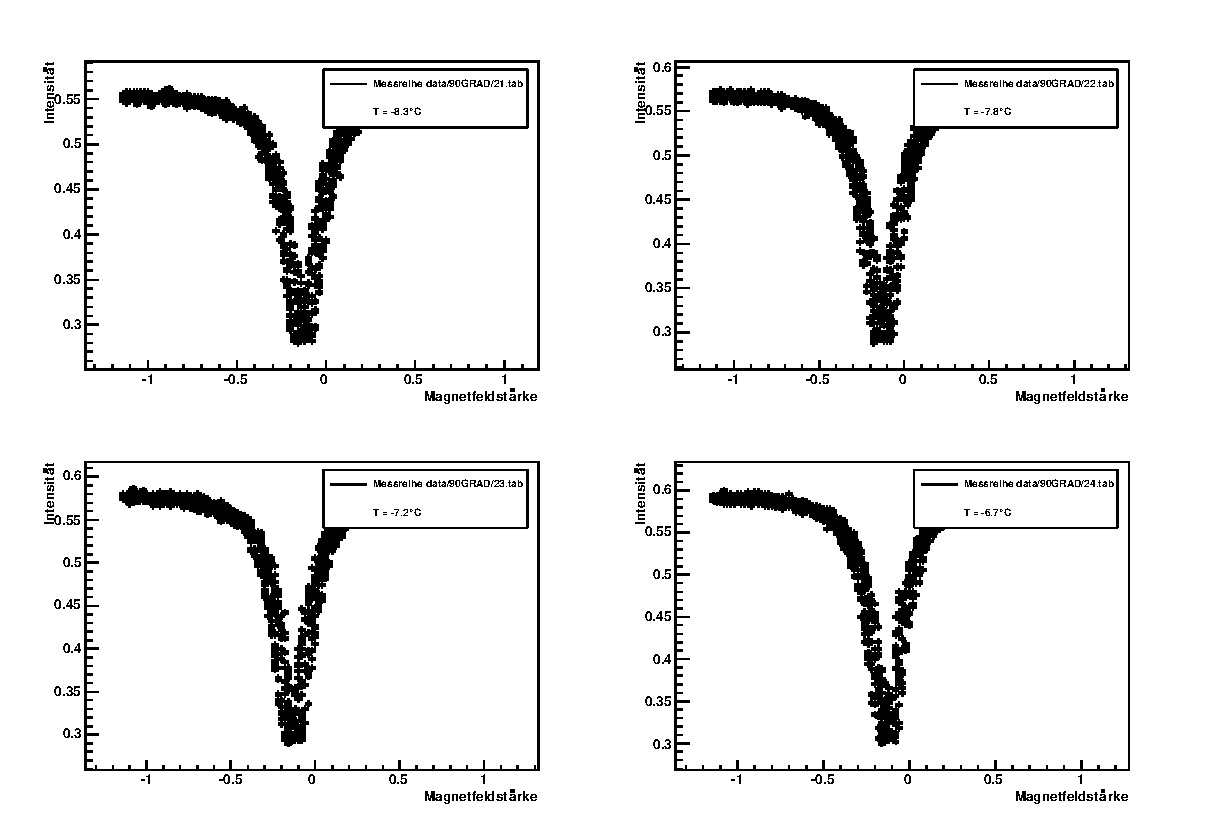
\includegraphics[width=1\linewidth]{pictures/2.eps} \\
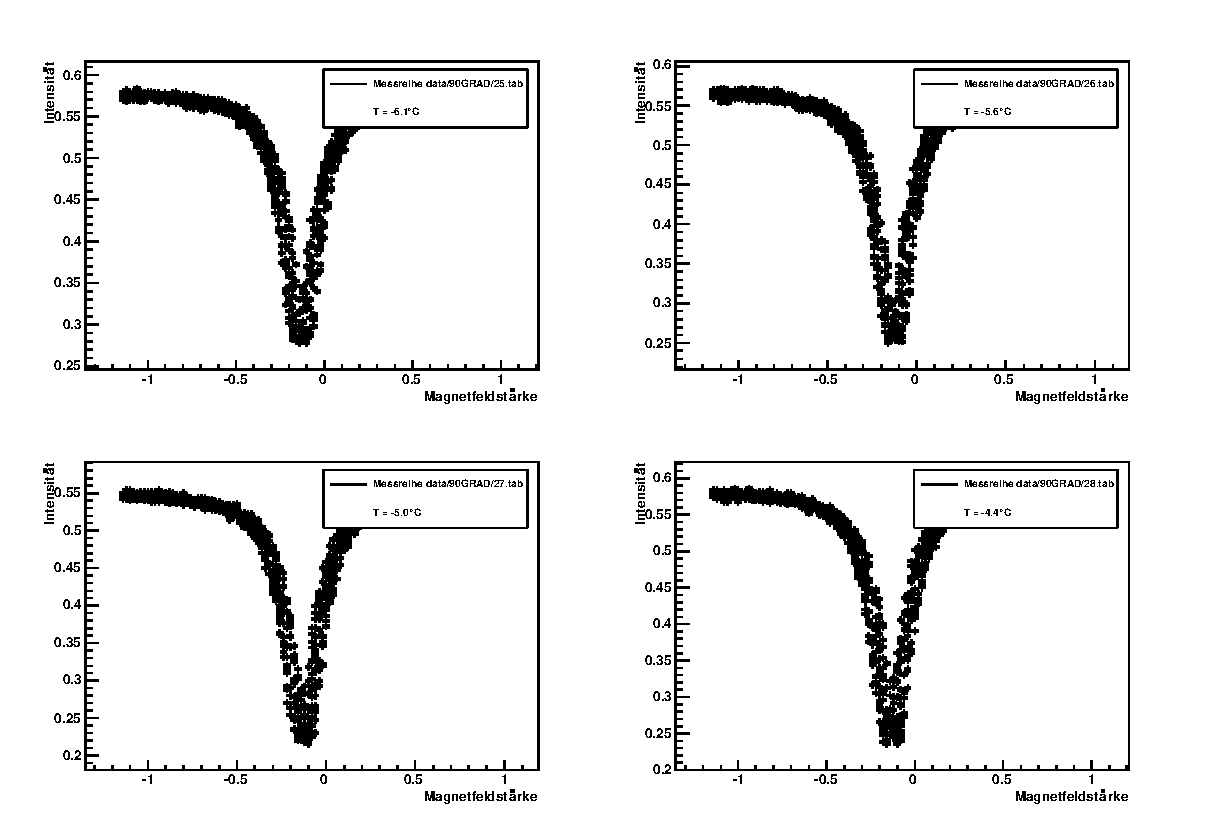
\includegraphics[width=1\linewidth]{pictures/3.eps} \\
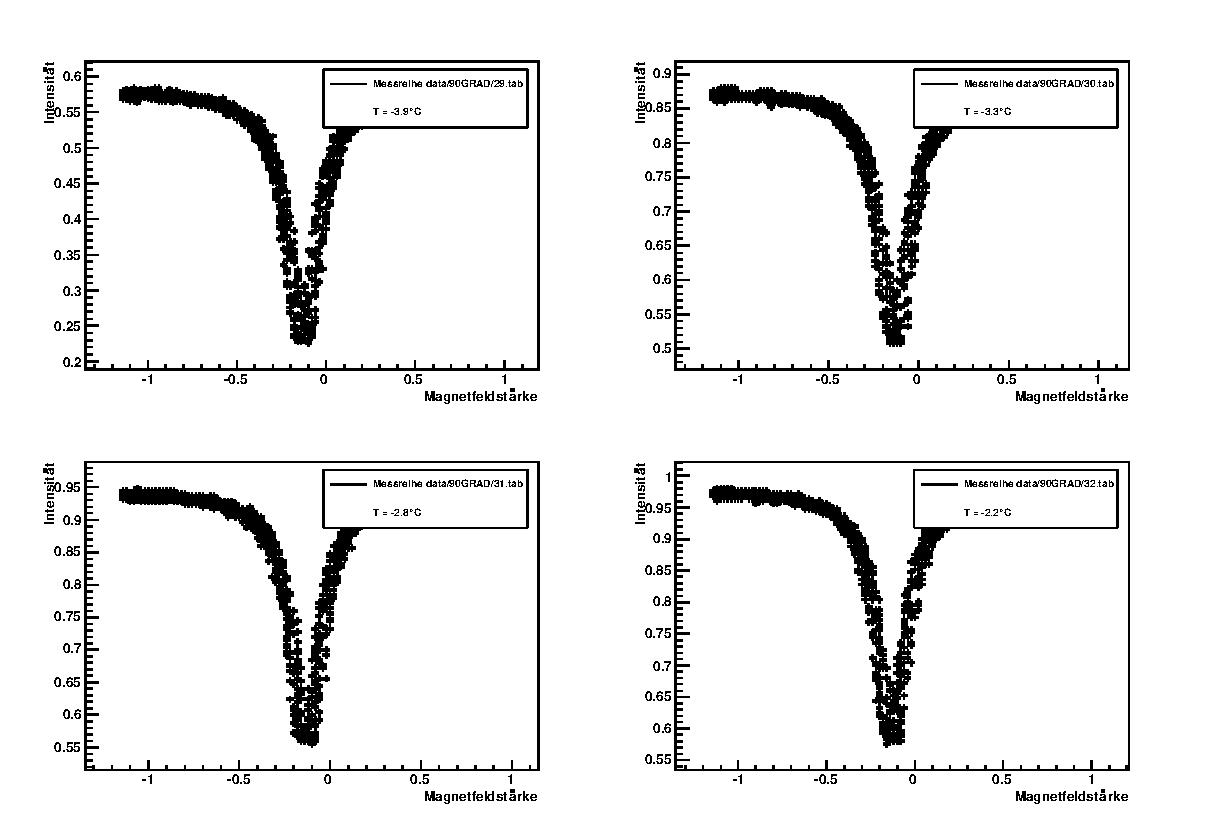
\includegraphics[width=1\linewidth]{pictures/4.eps} \\
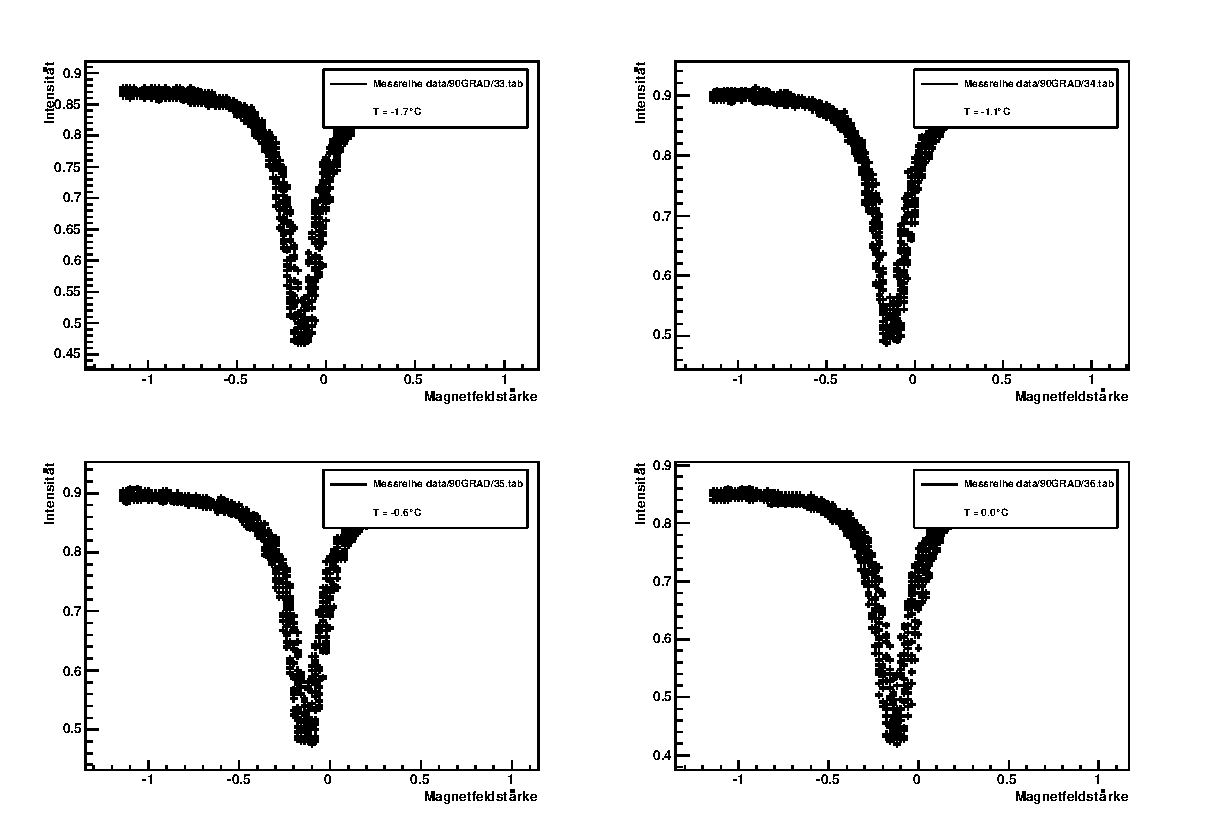
\includegraphics[width=1\linewidth]{pictures/5.eps} \\
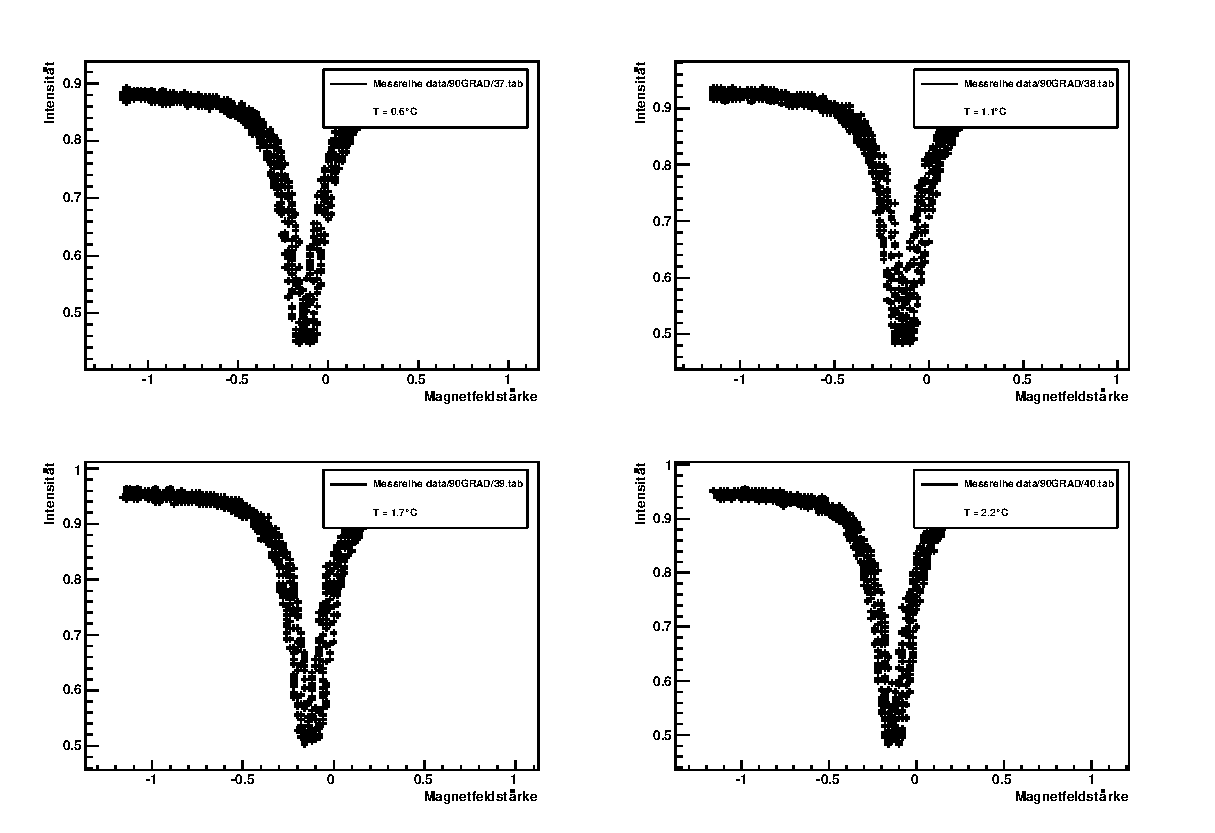
\includegraphics[width=1\linewidth]{pictures/6.eps} \\
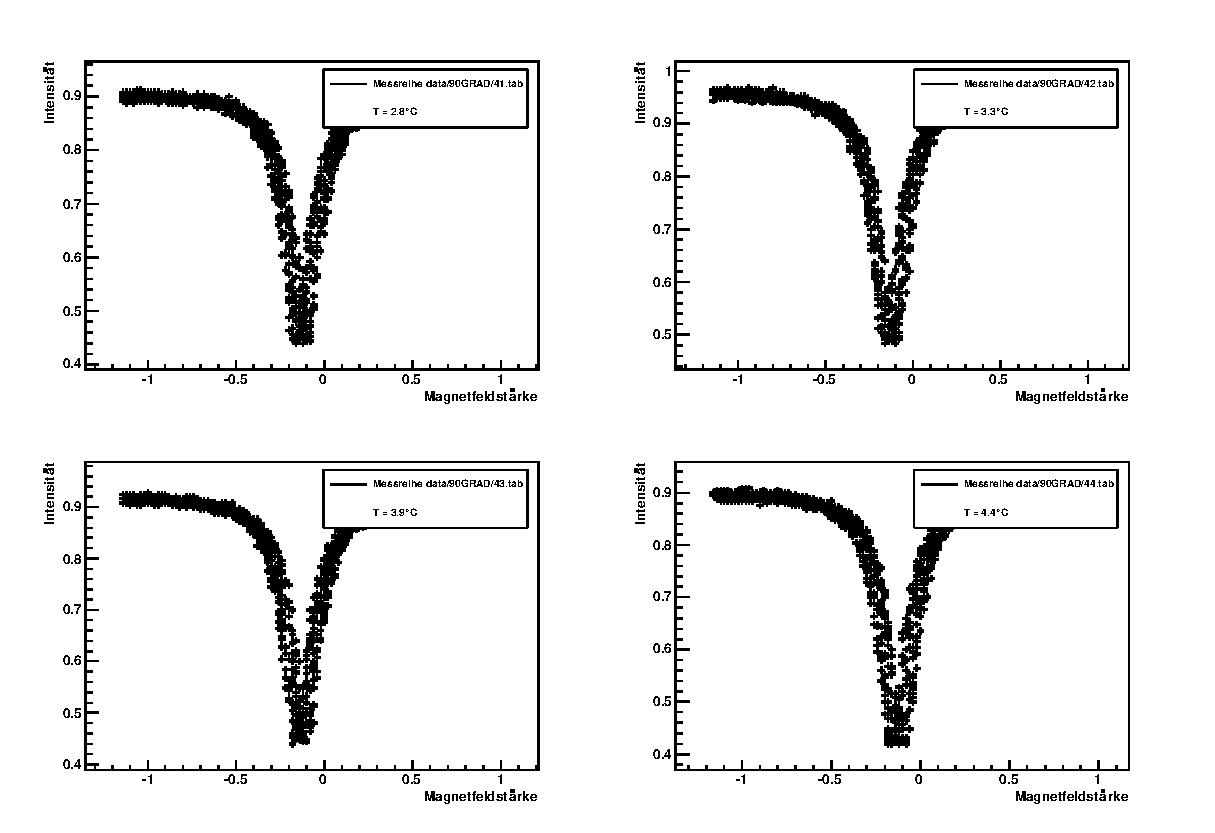
\includegraphics[width=1\linewidth]{pictures/7.eps} \\
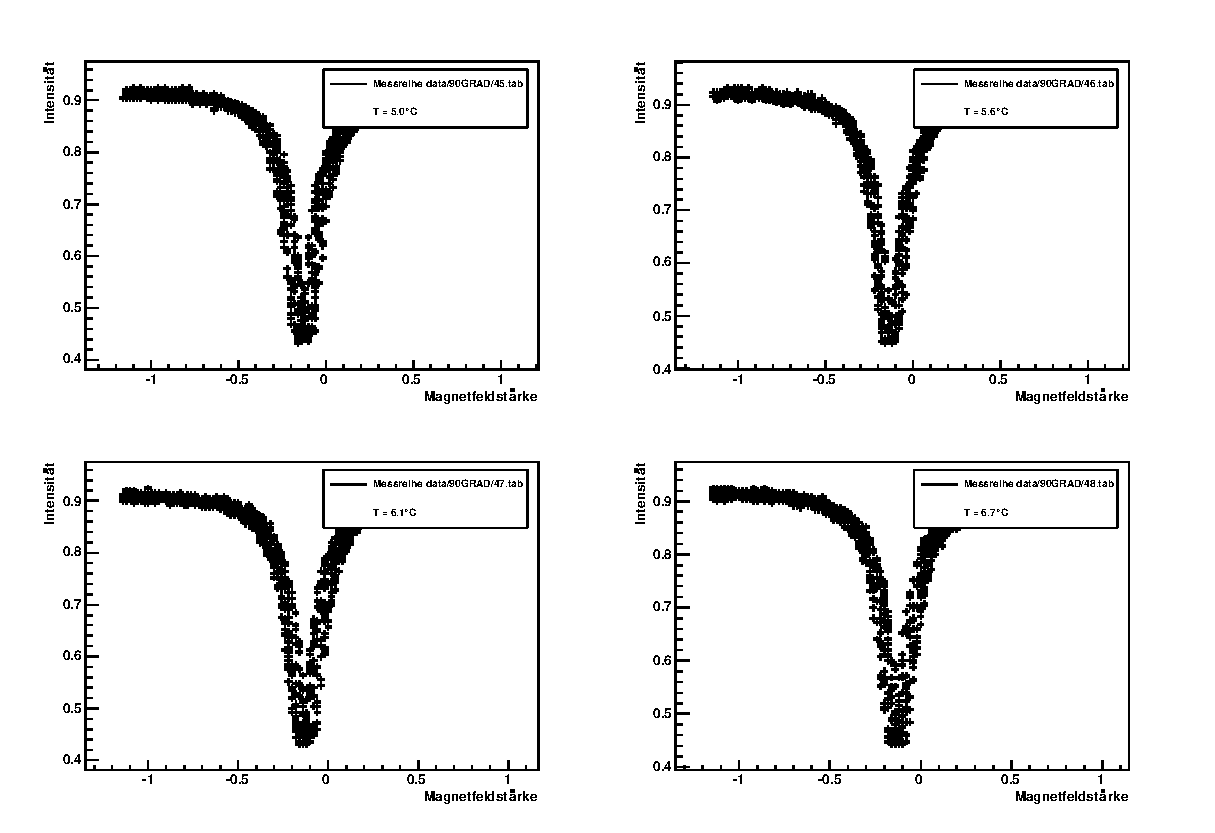
\includegraphics[width=1\linewidth]{pictures/8.eps} \\
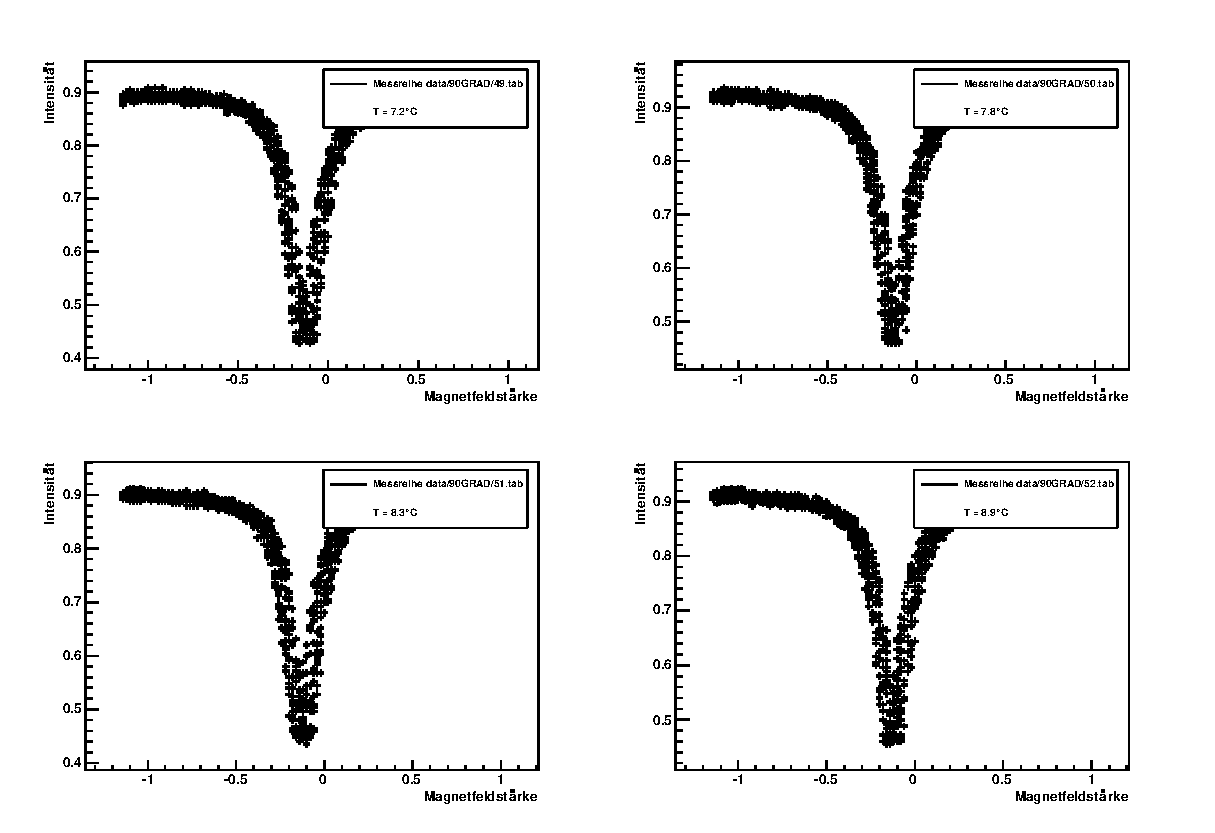
\includegraphics[width=1\linewidth]{pictures/9.eps} \\
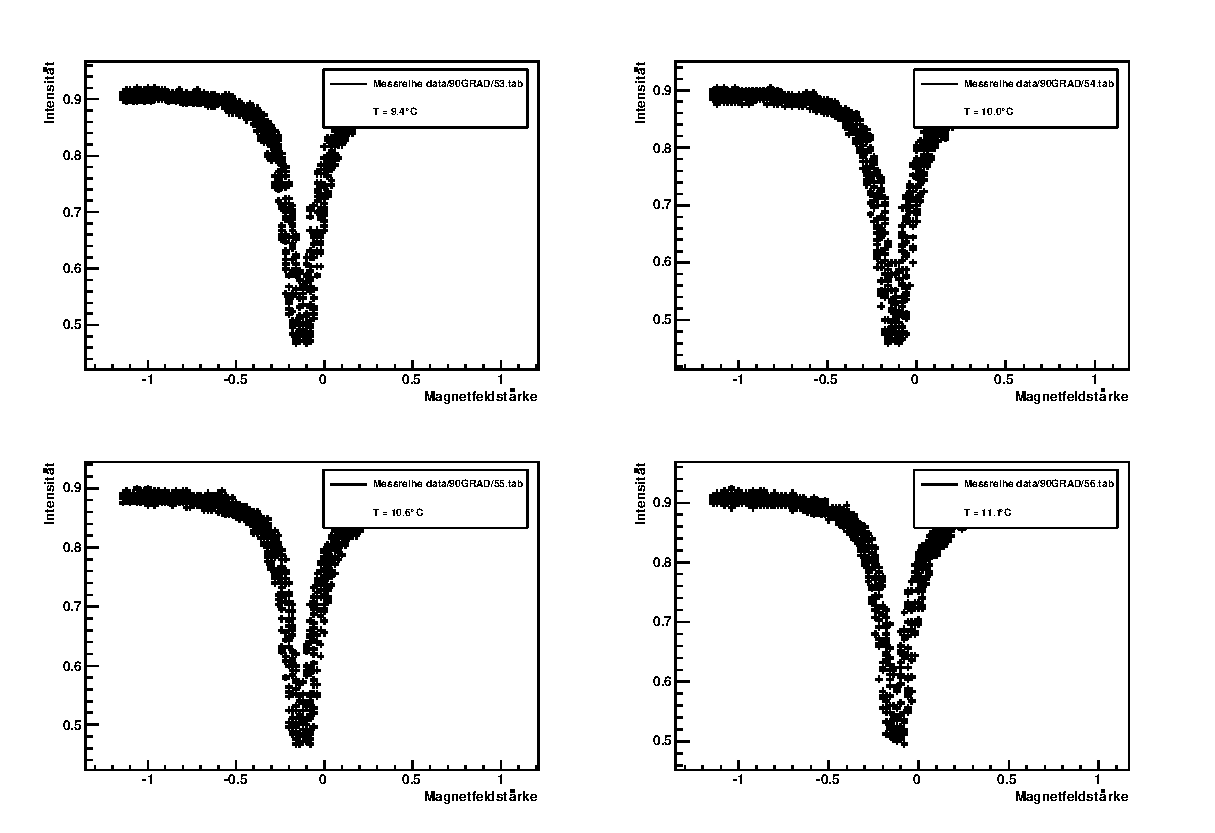
\includegraphics[width=1\linewidth]{pictures/10.eps} \\
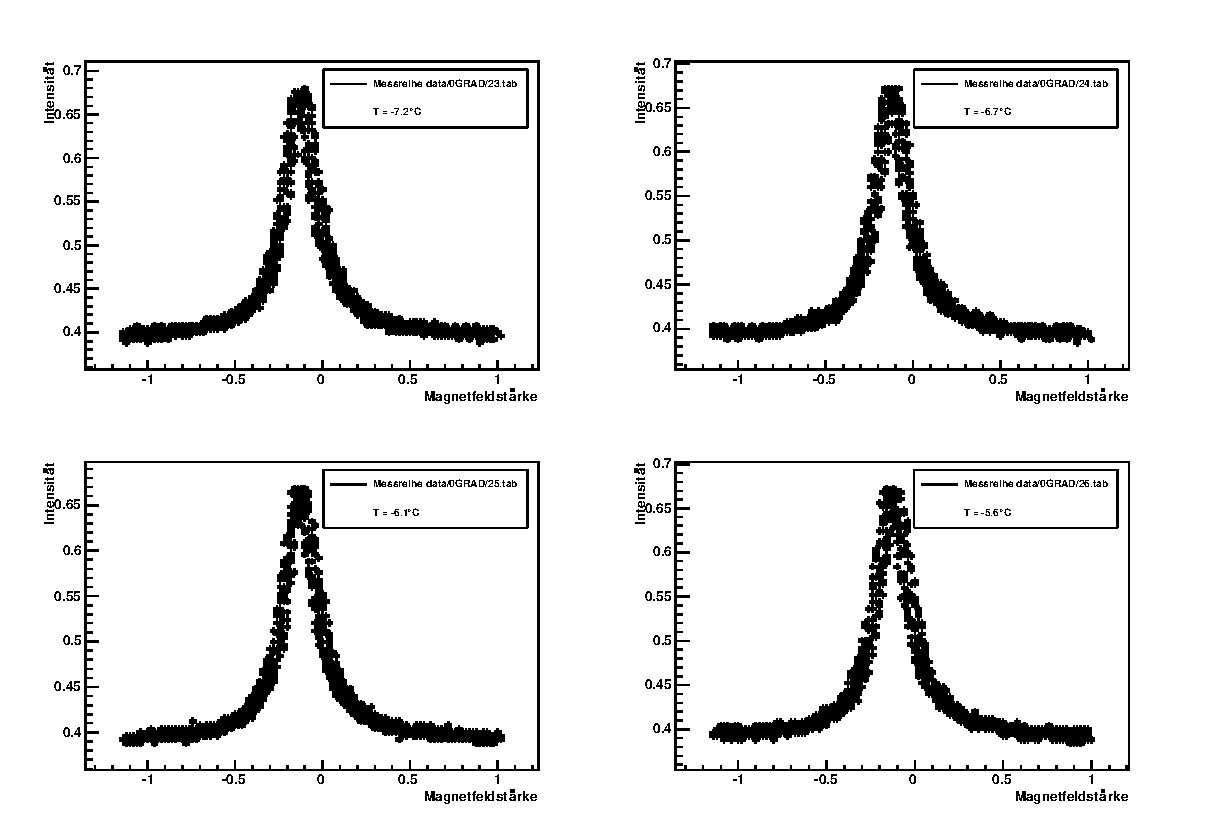
\includegraphics[width=1\linewidth]{pictures/11.eps} \\
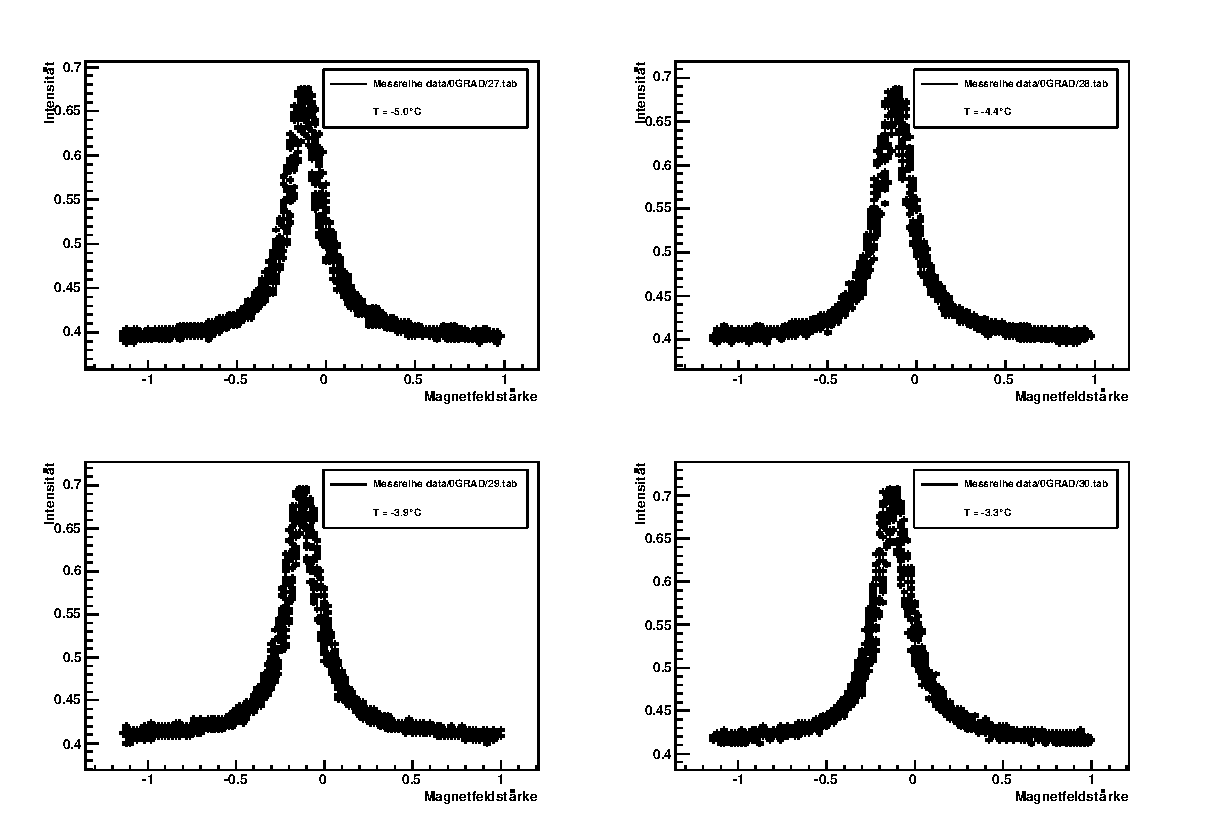
\includegraphics[width=1\linewidth]{pictures/12.eps} \\
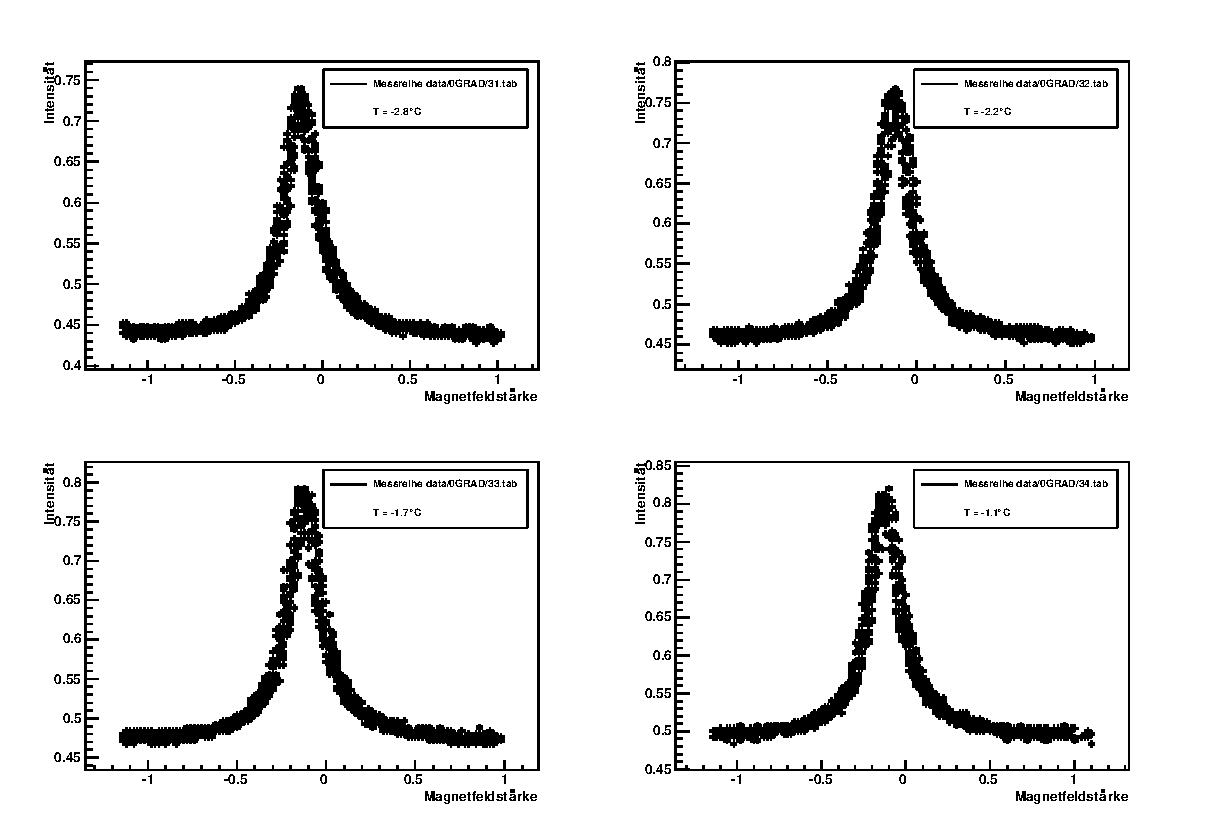
\includegraphics[width=1\linewidth]{pictures/13.eps} \\
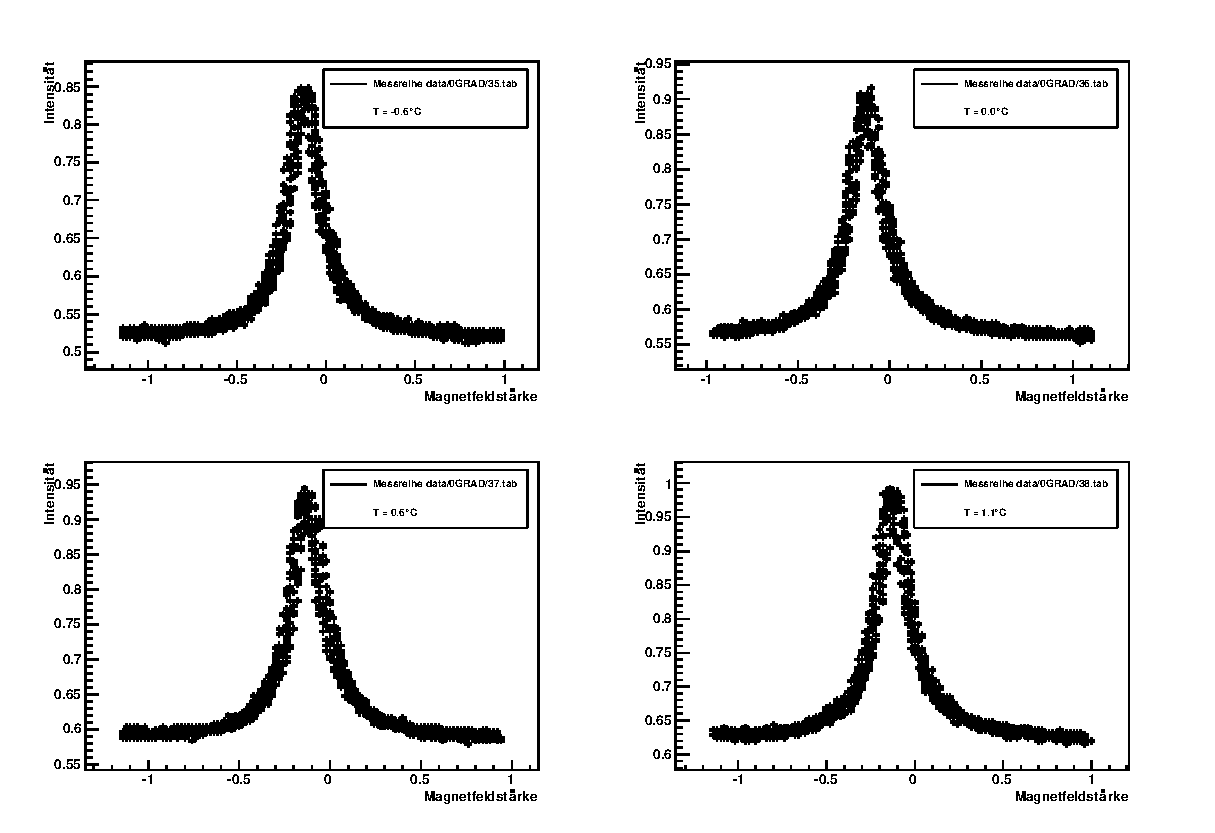
\includegraphics[width=1\linewidth]{pictures/14.eps} \\
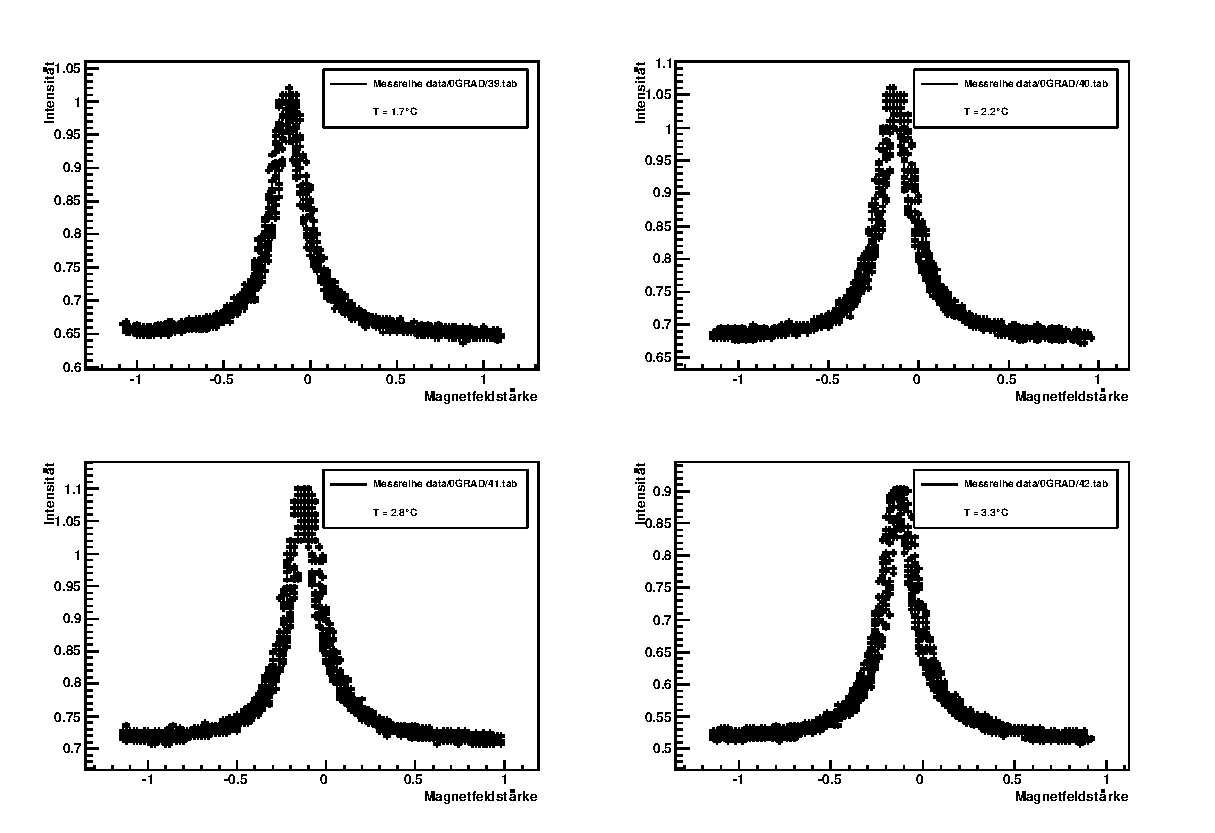
\includegraphics[width=1\linewidth]{pictures/15.eps} \\
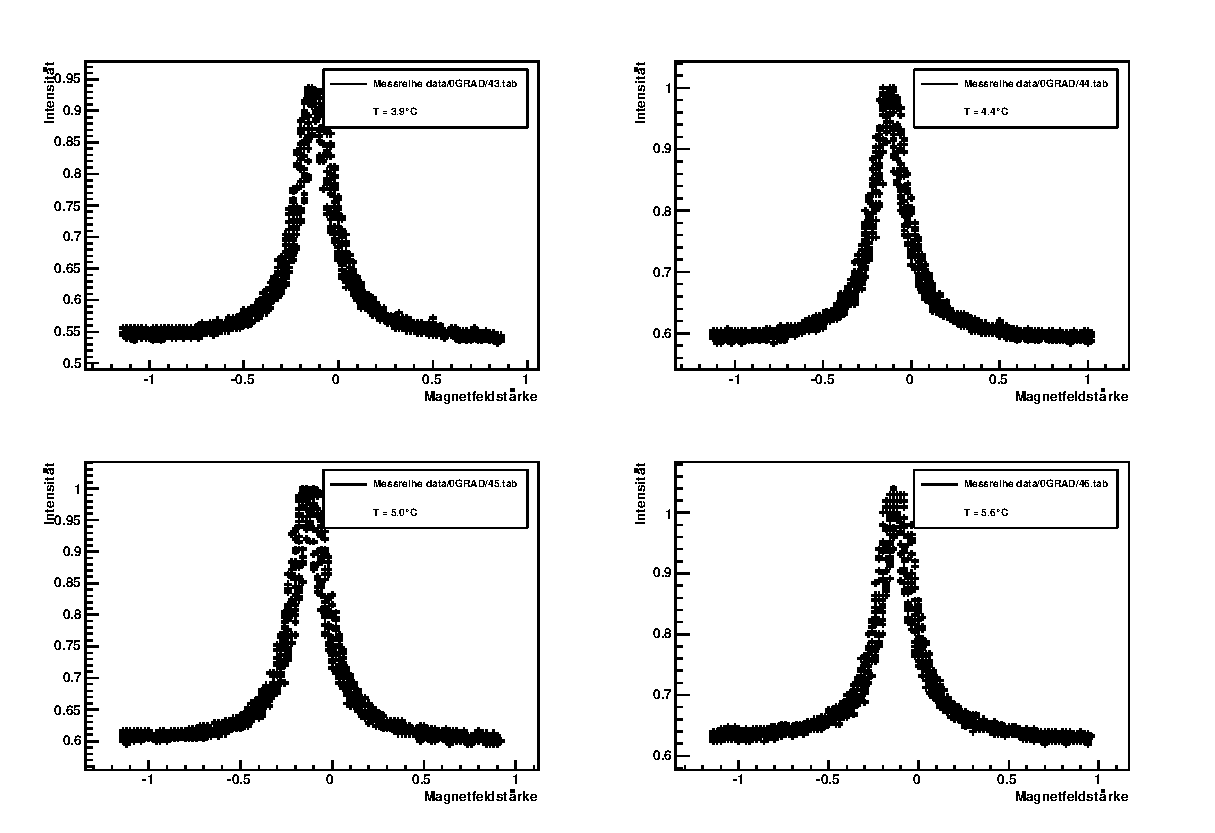
\includegraphics[width=1\linewidth]{pictures/16.eps} \\
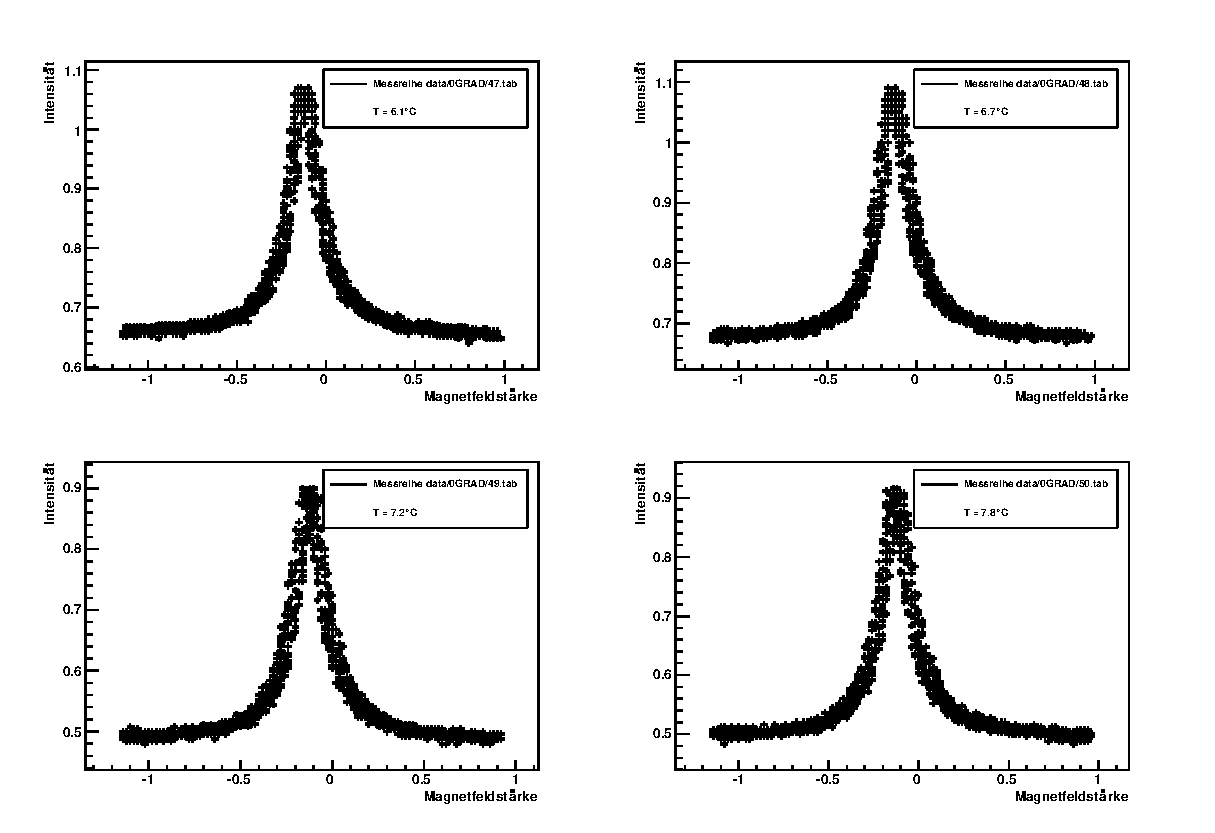
\includegraphics[width=1\linewidth]{pictures/17.eps} \\
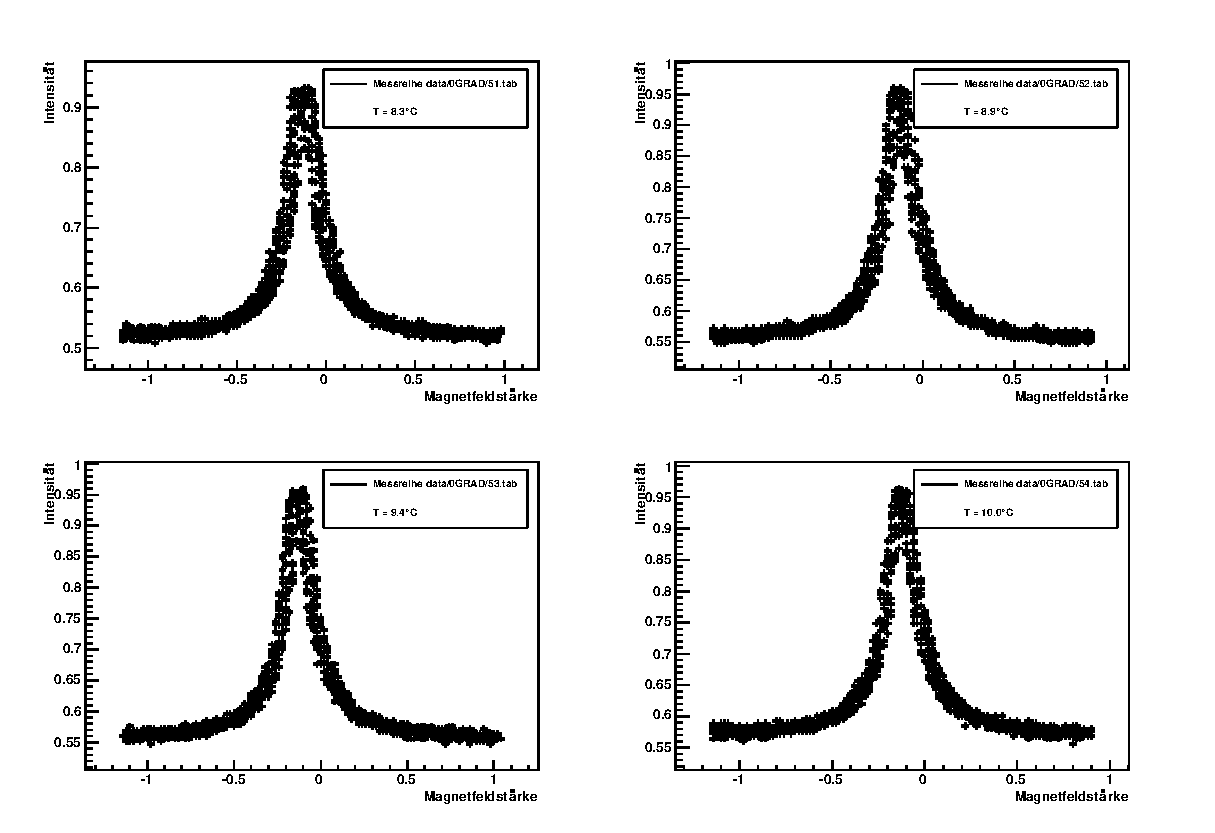
\includegraphics[width=1\linewidth]{pictures/18.eps} \\
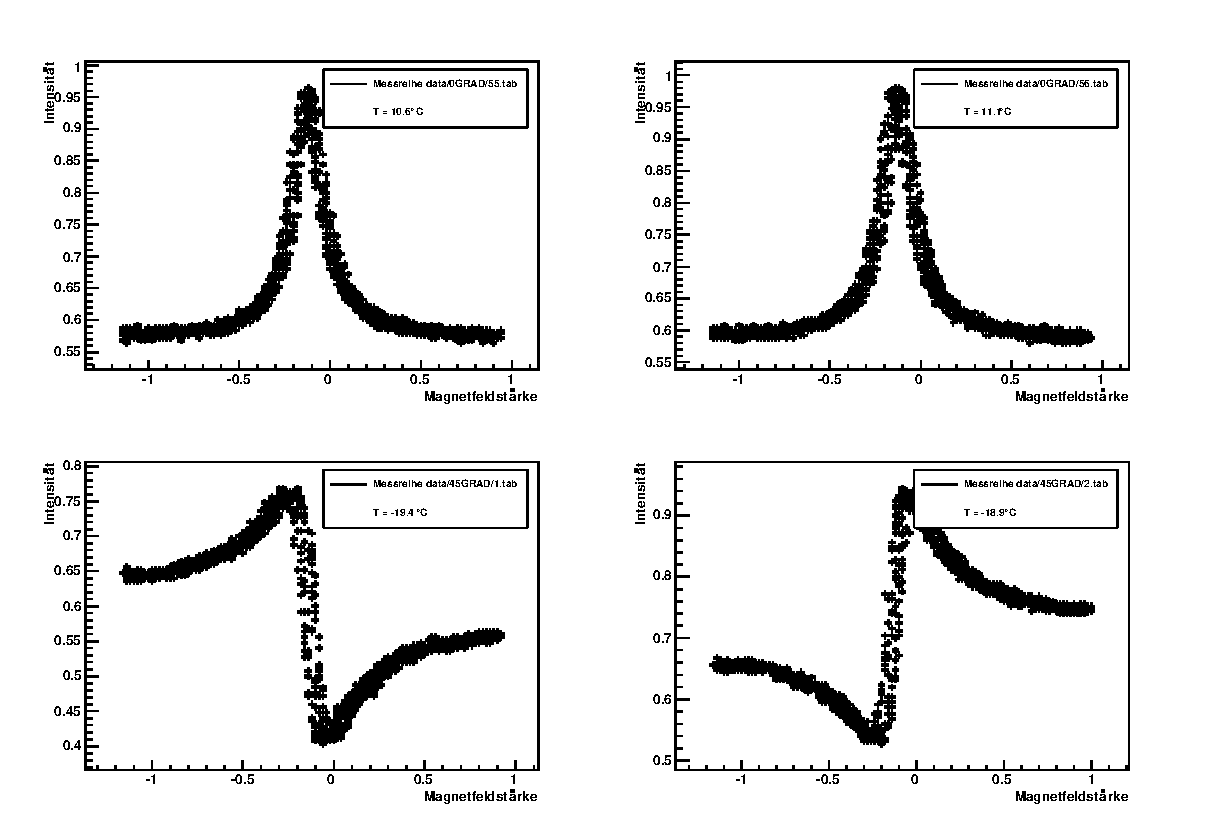
\includegraphics[width=1\linewidth]{pictures/19.eps} \\
\end{document}
